\documentclass[12pt]{article}
\usepackage[utf8]{inputenc}
\usepackage{geometry}
\usepackage{graphicx}
\usepackage{hyperref}
\usepackage{amsmath}
\usepackage{amsfonts}
\usepackage{listings}
\usepackage{xcolor}
\usepackage{float}
\usepackage{longtable}
\usepackage{array}
\usepackage{tabularx}
\usepackage{booktabs}
\usepackage{caption}
\usepackage{url}
\usepackage{tikz}
\usetikzlibrary{shapes.geometric, arrows, positioning, matrix}
\usepackage[document]{ragged2e}
\usepackage{pgfplots}
\tikzstyle{startstop} = [rectangle, rounded corners, minimum width=3cm, minimum height=1cm,text centered, draw=black, fill=red!30]
\tikzstyle{io} = [trapezium, trapezium left angle=70, trapezium right angle=110, minimum width=3cm, minimum height=1cm, text centered, draw=black, fill=blue!30]
\tikzstyle{process} = [rectangle, minimum width=3cm, minimum height=1cm, text centered, draw=black, fill=orange!30]
\tikzstyle{decision} = [diamond, minimum width=3cm, minimum height=1cm, text centered, draw=black, fill=green!30]
\tikzstyle{arrow} = [thick,->,>=stealth]

% Document geometry
\geometry{a4paper, margin=1in}

\title{
    {\Huge Software Requirements Specification} \\
    {\Large for} \\
    {\Large Angry Birds Alike} \\
    \vspace{0.5em}
    {\Large Author: Al Jubair Hossain} \\
    \vspace{0.5em}
    {\large Date: March 31, 2024}
}
\date{}

\begin{document}

\maketitle

\newpage

\section*{Revision History}
\begin{longtable}{|p{2cm}|p{2cm}|p{10cm}|}
    \hline
    \textbf{Date} & \textbf{Version} & \textbf{Notes} \\
    \hline
    Feb 3, 2024 & 1.0 & Initial draft completed. \\\hline
    February 26, 2024 & 1.5 & A fixed version with sections of 1.4, 4.1, 4.2, 5 were modified with specific information of physics computations. \\\hline
    March 31, 2024 & 2.0 & Final draft was completed with proposing methods for calculation ,and changes in all the sections of 3, 4.1-4.5.5, 5 ,9, 10 , 12 , 13, 16 ,17,19,20, 21 ,22, Appendix with specific info that was proposed in the project. Also, added the table of contents correctly and then adding all the formula and methods incorporating with the project . \\
    \hline
\end{longtable}

\newpage

\tableofcontents

\newpage

\section{Reference Material}
This section records information for easy reference, providing a foundation for the document's contents and ensuring a common understanding of terms and units used throughout.

\subsection{Table of Units}
Given the focus on physics simulations in the game, the following units are primarily used:

\begin{table}[H]
\centering
\begin{tabular}{|l|l|l|}
\hline
\textbf{Symbol} & \textbf{Unit} & \textbf{Description} \\
\hline
m & Meter & Unit of length, significant for distance calculations in simulations \\
kg & Kilogram & Unit of mass, crucial for force and momentum calculations \\
s & Second & Unit of time, used for time-stepping in physics simulations \\
m/s & Meter per Second & Unit of velocity, describing the speed of objects \\
m/s$^2$ & Meter per Second Squared & Unit of acceleration, including gravity \\
N & Newton & Unit of force, applicable in simulations involving collisions \\
rad & Radian & Unit for angular measurements, used in trajectory angles \\
\hline
\end{tabular}
\caption{Primary Units used in the document}
\label{table:units_corrected}
\end{table}

\subsection{Table of Symbols}
This document uses various symbols to describe physical quantities:

\begin{table}[H]
\centering
\begin{tabular}{|l|l|l|}
\hline
\textbf{Symbol} & \textbf{Unit} & \textbf{Description} \\
\hline
$v$ & m/s & Velocity \\
$a$ & m/s$^2$ & Acceleration \\
$F$ & N & Force \\
$m$ & kg & Mass \\
$g$ & m/s$^2$ & Acceleration due to gravity \\
\hline
\end{tabular}
\caption{Symbols and their descriptions}
\label{table:symbols}
\end{table}

\subsection{Abbreviations and Acronyms}
The document utilizes various abbreviations and acronyms to streamline discussion:

\begin{table}[H]
\centering
\begin{tabular}{|l|l|}
\hline
\textbf{Abbreviation/Acronym} & \textbf{Meaning} \\
\hline
SRS & Software Requirements Specification \\
RK4 & Runge-Kutta 4th Order Method \\
SI & International System of Units \\
AB\_Sim & Angry Birds Alike Simulation \\
\hline
\end{tabular}
\caption{Abbreviations and acronyms}
\label{table:abbreviations}
\end{table}

\subsection{Mathematical Notation}
The document employs mathematical notation consistent with physics and engineering principles, where:
- Scalars (e.g., mass, time) are denoted in italic (e.g., \(m\), \(t\)).
- Vectors (e.g., velocity, force) are represented in bold (e.g., \(\mathbf{v}\), \(\mathbf{F}\)).
- Differential equations and formulas integral to the game's physics engine are presented in standard mathematical format, facilitating clear communication of algorithms and methods, such as the Runge-Kutta 4 (RK4) method for numerical integration.

\newpage

\section{Introduction}

\subsection{Purpose of Document}
This Software Requirements Specification (SRS) document delineates the comprehensive specifications for "Angry Birds Alike," a physics-based game simulation designed to offer both an engaging gaming experience and an educational platform for physics students and enthusiasts. The document serves as a foundational blueprint for the development team, outlining the game's intended functionalities, performance expectations, and user interaction paradigms. Additionally, it acts as a reference point for stakeholders to understand the project's scope, objectives, and technical constraints, facilitating a shared vision for the project's successful completion.

\subsection{Scope of Requirements}
"Angry Birds Alike" aspires to transcend traditional gaming boundaries by integrating rigorous physics simulations that mirror real-world dynamics. The game's scope includes the design and development of a physics engine capable of simulating force, trajectory, momentum transfer, and elastic collisions. Coupled with an intuitive user interface, the game aims to challenge players to apply principles of physics to navigate through levels creatively. This document captures all requisite features, from user interactions, graphical representations, physics calculations, to the system's performance and scalability. It encompasses both functional and non-functional requirements essential for delivering a comprehensive and immersive gaming and learning experience.

\subsection{Characteristics of Intended Reader}
The intended audience for this document encompasses a broad spectrum of readers, including software developers, game designers, project managers, educational content creators, and stakeholders with vested interests in educational technology. A foundational understanding of software development processes, basic physics concepts, and game design principles is assumed. The document is structured to be accessible to readers with varying levels of technical expertise, providing both high-level overviews and detailed technical specifications.

\subsection{Organization of Document}
This document is organized into several key sections to facilitate ease of navigation and comprehension:

- **General System Description:** Outlines the high-level overview of the game, including its context, user characteristics, and system constraints.\\
- **Specific System Description:** Delves into the detailed problem statement, theoretical models, data definitions, and solution characteristics.\\
- **System Features and Requirements:** Enumerates the game's core functionalities, performance metrics, software attributes, and both functional and non-functional requirements.\\
- **Development Plan:** Provides a roadmap for the game's development lifecycle, including phases from initial requirements gathering to post-launch support.\\
- **Appendices:** Offers additional resources, such as a glossary of terms, user stories, compliance requirements, and detailed explanations of complex concepts like the RK4 method.


\section{General System Description}

This section provides a broad overview of the "Angry Birds Alike" system, detailing its main components, interfaces, user interactions, and operational constraints. It sets the stage for understanding the game's purpose, its interaction with users, and the environment in which it operates.

\subsection{System Context}

"Angry Birds Alike" is designed as a standalone application that engages users in physics-based puzzles. The system interacts with users through a graphical user interface (GUI), where players input actions via mouse or touchscreen gestures. The application processes these inputs to simulate and display physics-based trajectories and collisions. Data, such as level progress, scores, and user settings, are stored locally on the user's device. The game does not require an internet connection for core gameplay but may connect to online servers for updates, leaderboards, and sharing achievements.

\subsection{User Characteristics}

The primary users of "Angry Birds Alike" include individuals with an interest in physics, puzzle games, and educational software. The game is designed to be accessible to users of varying ages and educational backgrounds, from elementary students learning basic physics to adults seeking challenging puzzles. No specific technical skills are required to play the game, but users with a basic understanding of physics concepts may have an initial advantage.

\subsection{System Constraints and Limitations}

The game is developed to run on multiple platforms, including Windows, macOS, Android, and iOS, with considerations for the varying processing power and screen sizes. It is built with scalability in mind, allowing for the addition of new levels, physics simulations, and user interfaces without significant overhauls. However, the complexity of physics simulations is balanced with the need for the game to run smoothly on lower-end devices, which may limit the simulation's detail or the number of simultaneous interactions.

\subsection{Assumptions and Dependencies}

It is assumed that users have access to a device capable of running the game with a modern operating system. The game's performance and features depend on the device's hardware capabilities, such as CPU speed, graphics processing power, and available memory. Future versions of the game may depend on updates to third-party libraries such as SFML and Boost.odeint for graphical rendering and physics simulations.

\section{Specific System Description}

\subsection{Problem Description}
"Angry Birds Alike" simulates a vibrant, physics-based environment where players utilize principles of classical mechanics to solve puzzles. The challenge involves using a slingshot to launch birds with specific properties at structures, aiming to achieve maximum impact with strategic force and angle decisions. This scenario serves as an educational platform, promoting an intuitive understanding of physics concepts like projectile motion, elasticity, and conservation of energy.

\subsection{Terminology and Definitions}
This section introduces key terms that are essential for understanding the game's mechanics and physics simulations:

\subsection{Physics Engine and Game Mechanics}
The game's physics engine is designed to simulate realistic interactions based on classical mechanics principles. Utilizing the Runge-Kutta 4th Order Method (RK4) for numerical integration, the engine accurately predicts projectile trajectories, collision outcomes, and object movements under gravitational forces.

\subsubsection{Theoretical Background}
The engine incorporates several key physics concepts:
\begin{itemize}
    \item Projectile Motion: Calculated using $v_0$, launch angle $\theta$, and gravitational acceleration $g$, to determine trajectory.
    \item Collisions: Simulates elastic and inelastic collisions, applying conservation of momentum and energy principles.
    \item Gravity Effects: All objects are subjected to gravitational forces, influencing their motion.
\end{itemize}

\subsubsection{Implementation Details}
The physics engine is implemented in C++ with the Boost.odeint library for solving differential equations. Key formulas include:
\begin{align}
    \frac{dy}{dt} &= v \\
    \frac{dv}{dt} &= -g \\
    y(t) &= y_0 + v_0t + \frac{1}{2}gt^2
\end{align}
These equations form the basis for calculating object positions over time.


\begin{description}
\item[Projectile Motion:] Describes the motion of an object thrown into space upon which external forces, such as gravity, act.
\item[Elastic Collision:] A type of collision where the total kinetic energy of the colliding bodies after interaction is equal to their kinetic energy before interaction, ideal for understanding energy conservation.
\item[Momentum:] A measure of the motion of a body, equal to the product of its mass and velocity. Momentum conservation is a fundamental concept in collisions.
\item[Runge-Kutta 4 Method (RK4):] A numerical method used to approximate solutions to ordinary differential equations, critical for simulating precise projectile trajectories and other physics phenomena in the game.
\end{description}

\subsection{Physical System Description}
The game world comprises the following physical elements, each interacting according to the laws of physics:

Projectiles (Birds): Characters with unique masses and sizes, used by players to hit targets.
Targets (Pigs): Objects to be hit by the projectiles, often protected by various structures.
Obstacles: Various structures built from materials with different properties (wood, ice, stone) affecting the projectile's trajectory and collision outcomes.
\subsection{Goal Statements}
The primary goals of "Angry Birds Alike" include:

GS1: To provide a realistic physics simulation that allows players to apply and observe principles of projectile motion, force, and momentum in a fun and engaging way.
GS2: To offer a challenging puzzle game where players must use strategic thinking and a basic understanding of physics to progress through levels.
GS3: To create an educational tool that enhances the player's understanding of physics through interactive gameplay and immediate feedback on the physical consequences of their actions.
\subsection{Solution Characteristics Specification}

\subsubsection{Assumptions}

The game's physics engine can simulate real-world physics with high accuracy within computational constraints.
Players possess or will develop a basic understanding of physics principles through gameplay.
The user's device has sufficient processing power to handle real-time physics calculations and graphics rendering.
\subsubsection{Theoretical Models}
The game's physics engine integrates several theoretical models to simulate realistic interactions:

Projectile Motion Model (TM1): Determines the trajectory of birds based on initial force and angle, incorporating air resistance at higher levels.
Elastic Collision Model (TM2): Calculates energy and momentum transfer during collisions, providing the basis for interactions between birds, pigs, and obstacles.
Gravity Model (TM3): Applies a constant acceleration downwards, affecting all non-static objects in the game environment.
\subsubsection{Data Definitions}
Key data elements used in the game's physics calculations include:

Initial Conditions (DD1): Position, velocity, and mass of projectiles at the start of their trajectory.
Material Properties (DD2): Density, elasticity, and friction coefficients for different obstacle materials, influencing collision outcomes.
\subsubsection{Instance Models}
Specific instances where theoretical models are applied to simulate game scenarios:

Trajectory Calculation (IM1): Utilizes TM1 to predict and animate the flight path of projectiles in real-time.
Collision Detection and Response (IM2): Employs TM2 and TM3 to detect when and how projectiles interact with targets and obstacles, calculating the outcome based on physics principles like conservation of momentum and energy transfer.

\subsubsection{Environment Interaction (IM3):}
Factors in external influences such as wind or gravitational variations in special levels, adjusting projectile trajectories and collision impacts accordingly, introducing complex scenarios for players to strategize around.

\section{System Features}

This section outlines the major features of "Angry Birds Alike", detailing how each contributes to the gameplay experience and educational value of the game. These features are designed to engage players in physics concepts through interactive and challenging gameplay.

\subsection{Projectile Simulation}
\textbf{Description:} This feature allows players to control the angle and velocity of projectiles (birds) launched at targets (pigs). The simulation includes real-world physics considerations such as gravity, drag, and the material properties of obstacles.

\textbf{Functional Requirements:}
\begin{itemize}
    \item Players must be able to adjust the launch angle and force applied to the projectile.
    \item The game will calculate the projectile's trajectory using the Runge-Kutta 4 method for accurate physics simulation.
    \item Collisions with targets and obstacles must reflect realistic physics interactions.
\end{itemize}

\subsection{Level Design and Physics Challenges}
\textbf{Description:} Levels are designed to introduce players to various physics concepts, including projectile motion, elasticity, and momentum conservation. Each level presents unique challenges that require players to apply physics principles to solve.

\textbf{Functional Requirements:}
\begin{itemize}
    \item Levels progressively increase in difficulty to match the player's understanding and skills.
    \item The game provides visual and textual hints related to the physics concepts explored in each level.
    \item Success criteria for levels are based on physics objectives, such as knocking down structures or reaching specific targets.
\end{itemize}

\subsection{Interactive Physics Sandbox}
\textbf{Description:} An open-ended mode where players can experiment with different physics setups. This sandbox feature serves as both a playground and a learning tool, enabling players to explore physics principles without the constraints of structured levels.

\textbf{Functional Requirements:}
\begin{itemize}
    \item Provide a variety of objects, materials, and environmental conditions for players to experiment with.
    \item Allow players to adjust variables such as gravity, air resistance, and object properties.
    \item Include tools for measuring and displaying velocities, forces, and trajectories to facilitate learning.
\end{itemize}

\subsection{Educational Content and Tutorials}
\textbf{Description:} To enhance the game's educational value, this feature includes tutorials and in-game explanations of the physics principles at play. It aims to bridge the gap between gameplay and learning, making complex concepts accessible and engaging.

\textbf{Functional Requirements:}
\begin{itemize}
    \item Tutorials must clearly explain how to play the game and how physics is integrated into the gameplay.
    \item In-game content should include explanations of physics concepts, examples, and real-world applications.
    \item The game should offer feedback on the player's actions, highlighting the physics principles involved in their successes and failures.
\end{itemize}

\section{Performance Requirements}
\begin{itemize}
    \item The game shall maintain a high frame rate for smooth animations during simulations.
    \item Physics calculations for projectile motion and collisions shall be computed in real-time to provide immediate feedback to player actions.
\end{itemize}

\section{Software System Attributes}
\subsection{Reliability}
The game shall have error handling for user inputs and unexpected behaviors to prevent crashes and ensure
\section{Software System Attributes}
\subsection{Reliability}
The game shall have error handling for user inputs and unexpected behaviors to prevent crashes and ensure consistent performance across various platforms.

\subsection{Maintainability}
Code shall be well-documented and modular to facilitate easy updates and incorporation of new physics models or game features.

\subsection{Portability}
The game will be developed to run on various operating systems including Windows, macOS, and Linux without requiring significant changes to the codebase.

\section{Technological Overview}
\subsection{SFML}
SFML provides a simple interface to the various components of a PC, simplifying the game development process and allowing for a focus on the game mechanics and physics.

\subsection{Boost.odeint}
Utilized for its advanced ODE solving capabilities, allowing for accurate and efficient simulation of the game's physics.

\subsection{C++ Standard Library}
Used for its robust performance and reliability, particularly the data structures, mathematical functions, and threading capabilities for managing the game's physics simulations.

\section{Physics Simulation Detail}
\subsection{Projectile Simulation}
\subsubsection{Runge-Kutta Method}
We use RK4 for trajectory prediction by numerically integrating the equations of motion. The game updates the state of the projectile based on the forces applied, such as the initial throw and gravity.

\subsection{Collision Detection and Response}
\subsubsection{Elastic Collision}
When a collision is detected between two entities, the game calculates the resulting velocities and direction changes according to the principles of elastic collision.

\subsubsection{Momentum Transfer}
Momentum conservation is applied to all collisions within the game to simulate realistic interactions between objects.

\section{Challenges and Improvements}
\subsection{Challenges}
\begin{itemize}
    \item Implementation of the RK4 method for accurate physics simulation.
    \item Creation of a robust stepper function for physics updates.
    \item Accurate momentum transfer in multi-object collisions.
    \item Efficient collision detection among multiple targets.
\end{itemize}

\subsection{Improvements}
\begin{itemize}
    \item Introduction of advanced computational logic such as piecewise functions for enhanced gameplay mechanics.
    \item Inclusion of additional physics elements such as wind forces and air resistance.
    \item Enhanced visual effects for a more immersive gaming experience.
    \item Addition of new levels and features, including time-limited challenges to increase game complexity.
\end{itemize}

\section{Functional Requirements}
The game must satisfy the following functional requirements:
\begin{enumerate}
    \item Provide accurate simulations of projectile motion using the RK4 method.
    \item Allow players to interactively control the angle and force of projectile launch.
    \item Simulate physics in real-time to provide immediate feedback.
    \item Include multiple levels with varying physics challenges.
    \item Implement a scoring system based on the efficiency and accuracy of hitting targets.
\end{enumerate}

\section{Non-functional Requirements}
The non-functional requirements of the game include:
\begin{enumerate}
    \item \textbf{Usability:} The game should be easy to learn but challenging to master.
    \item \textbf{Performance:} The game should run smoothly on all supported platforms with minimal loading times.
    \item \textbf{Accessibility:} The game should be accessible, following the WCAG guidelines where applicable.
\end{enumerate}

\section{Traceability Matrices and Graphs}

This section contains the traceability matrices that map system features to their corresponding requirements, design components, and instance models, ensuring comprehensive coverage and verification.

\subsection{Requirement to Instance Model Traceability Matrix}
This matrix correlates each requirement with the instance models and design elements that implement them.

\begin{longtable}{|p{0.15\linewidth}|p{0.4\linewidth}|p{0.15\linewidth}|p{0.2\linewidth}|}
\hline
\textbf{Req ID} & \textbf{Requirement Description} & \textbf{Instance Model(s)} & \textbf{Design Element(s)} \\
\hline
FR1 & Accurate projectile motion simulation & IM1 & Physics Engine \\
FR2 & Interactive control for projectile launch & IM1 & User Interface Module \\
FR3 & Real-time physics feedback during gameplay & IM1, IM2, IM3 & Simulation Module \\
FR4 & Multiple levels with varied physics challenges & IM1, IM2 & Level Design System \\
FR5 & Scoring system reflecting physics accuracy & IM2 & Scoring Algorithm \\
NFR1 & Ease of learning and gameplay challenge & -- & Tutorial System \\
NFR2 & Smooth operation on supported platforms & -- & Performance Optimization \\
NFR3 & Accessibility following WCAG guidelines & -- & Accessibility Features \\
\hline
\end{longtable}

\subsection{Design to Test Case Traceability Matrix}
This matrix ensures that all design elements are covered by the test cases.

\begin{longtable}{|p{0.2\linewidth}|p{0.5\linewidth}|p{0.2\linewidth}|}
\hline
\textbf{Design ID} & \textbf{Design Element Description} & \textbf{Test Case(s)} \\
\hline
DE1 & Physics Engine for simulating motion & TC01, TC02 \\
DE2 & User Interface or inputs for interaction & TC03 \\
DE3 & Simulation Module for gameplay feedback & TC04, TC05 \\
DE4 & Level Design System for various challenges & TC06 \\
DE5 & Scoring Algorithm for accuracy & TC07 \\
DE6 & Tutorial System for ease of learning & TC08 \\
DE7 & Performance Optimization for smooth operation & TC09 \\
DE8 & Accessibility Features for compliance & TC10 \\
\hline
\end{longtable}

Note: Test cases (TC) are not explicitly mentioned in the provided document. They should be detailed in the test plan or quality assurance documentation and then linked to this matrix.

\subsection{Design to Test Case Traceability Matrix Graph}
This graph ensures that all design element correlates with all the Traceability models.
\centering
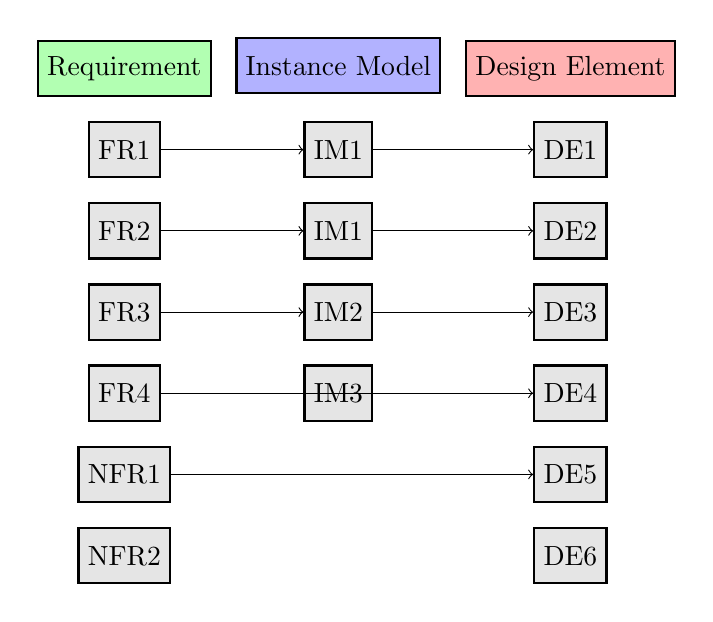
\begin{tikzpicture}
  \matrix (matrix) [matrix of nodes, nodes={draw, thick, fill=gray!20}, row sep=3mm, column sep=3mm, minimum height=2em] {
    |[fill=green!30]| Requirement & |[fill=blue!30]| Instance Model & |[fill=red!30]| Design Element \\
    FR1 & IM1 & DE1 \\
    FR2 & IM1 & DE2 \\
    FR3 & IM2 & DE3 \\
    FR4 & IM3 & DE4 \\
    NFR1 &  & DE5 \\
    NFR2 &  & DE6 \\
  };
  \draw[->] (matrix-2-1) -- (matrix-2-2);
  \draw[->] (matrix-2-2) -- (matrix-2-3);
  \draw[->] (matrix-3-1) -- (matrix-3-2);
  \draw[->] (matrix-3-2) -- (matrix-3-3);
  \draw[->] (matrix-4-1) -- (matrix-4-2);
  \draw[->] (matrix-4-2) -- (matrix-4-3);
  \draw[->] (matrix-5-1) -- (matrix-5-3);
  \draw[->] (matrix-6-1) -- (matrix-6-3);
\end{tikzpicture}

\RaggedRight
\section{Enhanced System Description}
Angry Birds Alike, inspired by the dynamics of "Angry Birds Game", is a sophisticated physics engine designed for educational simulations. It focuses on demonstrating intermediate to advanced physics mechanisms such as force, velocity, elastic collision, and momentum transfer. The engine utilizes mathematical formulas, specifically the Runge-Kutta 4 (RK4) method, to solve projectile trajectories accurately.

\subsection{Overview of Technologies}
\begin{itemize}
    \item \textbf{SFML (Simple and Fast Multimedia Library):} Utilized for window management, graphics rendering, and event handling.
    \item \textbf{Boost.odeint:} A comprehensive C++ library employed for solving ordinary differential equations (ODEs), crucial for simulating the physics interactions within the game.
    \item \textbf{C++ Standard Library Features:} Including Arrays for data management, cmath for mathematical calculations, chrono for managing time, and thread for optimizing performance through multi-threading.
\end{itemize}

\section{Physics Simulation Walkthrough}
The core of ProgName's simulation is built on accurately determining the trajectory of projectiles under various forces. This is achieved through the RK4 method, allowing for precise calculation of distances covered by the projectiles.

\subsection{RK4 Method Implementation}
Given the differential equations:

\[
\frac{dx}{dt} = vx, \quad \frac{dy}{dt} = vy, \quad \frac{dvx}{dt} = 0, \quad \frac{dvy}{dt} = g
\]

where \(g\) is the acceleration due to gravity. With initial conditions at \(t_0\) set as \(x_0 = 0\), \(y_0 = 0\), \(vx_0 = 10m/s\), and \(vy_0 = 10m/s\), we find the state after a timestep \(\Delta t = 1s\), applying the RK4 method.

\subsubsection{Projectile System Walkthrough}
This section details the calculation steps using RK4, from initial velocity setup to updating the state with a weighted average of the slopes (k values), and finally providing a summary of one timestep's calculation.

\section{Physics Mechanics Demonstrations}
\subsection{Force Application to Velocity}
Demonstrates the conversion of applied force into initial speed and direction, affecting the projectile's trajectory.\\
--Set the initial conditions for projectile motion by adjusting the launch angle (\(\theta\)) and the force (\(F\)), determining the initial velocity (\(v_0 = \frac{F}{m}\)), where \(m\) is the projectile's mass.

\subsection{Elastic Collision and Momentum Transfer}
Details the simulation of elastic collisions between entities, showcasing momentum conservation and transfer according to physics laws.\\
--Elastic collisions conserve both momentum and kinetic energy. For two colliding objects, momentum conservation is expressed as \(m_1v_{1,initial} + m_2v_{2,initial} = m_1v_{1,final} + m_2v_{2,final}\), and kinetic energy conservation as \(\frac{1}{2}m_1v_{1,initial}^2 + \frac{1}{2}m_2v_{2,initial}^2 = \frac{1}{2}m_1v_{1,final}^2 + \frac{1}{2}m_2v_{2,final}^2\).
    

\section{Challenges and Improvements}
\subsection{Challenges Faced}
\begin{itemize}
    \item Implementing the RK4 method for trajectory calculation.
    \item Developing a functional stepper function for physics updates.
    \item Accurate momentum transfer and collision detection among entities.
\end{itemize}

\subsection{Proposed Improvements}
\begin{itemize}
    \item Introduce more sophisticated computation logic, possibly utilizing piecewise functions or parametric equations to enrich the gameplay mechanics.
    \item Expand the physics simulations to include additional forces like wind and drag.
    \item Enhance visuals and user experience by adding diverse levels, implementing time-limits for launches, and refining the graphical interface.
\end{itemize}

\section{Pseudo Code for Physics Simulation}
\begin{lstlisting}[language=C++, caption={Physics System Simulation}, label={lst:physics_simulation}]
#include <boost/numeric/odeint.hpp>
#include <array>
// Define the state type for the simulation
using State = std::array<double, 4>; // x, y, vx, vy
using Stepper = boost::numeric::odeint::runge_kutta4<State>;

void projectileSystem(const State &state, State &dstate_dt, const double) {
    dstate_dt[0] = state[2]; // dx/dt = vx
    dstate_dt[1] = state[3]; // dy/dt = vy
    dstate_dt[2] = 0;        // dvx/dt = 0
    dstate_dt[3] = GRAVITY;  // dvy/dt = gravity
}
\end{lstlisting}

\section{Detailed Physical System Description}
Building on PS1 and PS2 from the Physical System Description, let's elaborate:

\begin{itemize}
    \item PS1: The simulation engine represents a physical environment where forces such as gravity, tension, and friction are simulated in real time to affect objects within the game.
    \item PS2: The user interface includes a viewport of the simulation, input controls for adjusting force and angle, and feedback displays for velocity and trajectory.
\end{itemize}

\section{Enhanced Solution Characteristics Specification}
\subsubsection{Assumptions}
\begin{itemize}
    \item[A3:] The system shall have access to sufficient computational resources to perform real-time simulations.
    \item[A4:] The user's input device is accurate and allows for precise control over input parameters.
\end{itemize}

\subsubsection{Enhanced Data Definitions}
In addition to DD1 and DD2, we consider:
\begin{itemize}
    \item[DD3:] Environmental Data - Includes parameters like wind speed and direction that affect the trajectory of projectiles.
\end{itemize}

\subsubsection{Enhanced Instance Models}
Building on IM1 and IM2:
\begin{itemize}
    \item[IM3:] Wind Influence Model - Integrates environmental data to adjust the projectile's trajectory accordingly.
\end{itemize}

\section{Enhanced Requirements}
\subsection{Additional Functional Requirements}
\begin{enumerate}
    \setcounter{enumi}{4}
    \item The system shall simulate the impact of environmental factors like wind on projectile trajectories.
    \item The system shall provide a tutorial mode that explains the physics concepts through interactive examples.
\end{enumerate}

\subsection{Additional Non-functional Requirements}
\begin{enumerate}
    \setcounter{enumi}{3}
    \item \textbf{Scalability:} The game shall be designed to easily integrate new physics models and game levels.
\end{enumerate}

\section{Additional System Features}
\subsection{Environmental Effects Simulation}
\begin{enumerate}
    \item The game will simulate environmental effects, providing players with challenges such as compensating for wind when aiming projectiles.
\end{enumerate}

\section{User Documentation and Help System}
\begin{enumerate}
    \item Comprehensive user documentation will be provided, explaining how to play the game and understand the underlying physics concepts.
    \item An in-game help system will offer hints and explanations for each level, aiding users in comprehending the application of physics in gameplay.
\end{enumerate}

\section{Development Plan}
The development of "Angry Birds Alike" will follow these phases:
\begin{enumerate}
    \item Requirements analysis and project setup.
    \item Core physics engine and gameplay mechanics development.
    \item Implementation of user interface and graphics.
    \item In-depth testing across platforms, fine-tuning based on feedback.
    \item Final preparations for launch, including marketing and creation of support documentation.
    \item Post-launch support and development of additional content based on user feedback.
\end{enumerate}

\section{Traceability Information and Coverage }
This matrix links SRS requirements, MG modules, and VnV test cases to ensure comprehensive coverage and coherence across documentation.

\begin{table}[H]
\centering
\begin{tabular}{|l|l|l|}
\hline
\textbf{SRS Requirement} & \textbf{MG Module} & \textbf{VnV Test Case} \\
\hline
IM1: Projectile Motion & M4: Physics Engine & TC1: Projectile Motion Accuracy \\
IM2: Collision Dynamics & M4: Physics Engine & TC2: Collision Dynamics \\
IM3: Gravity Effects & M4: Physics Engine & TC1: Gravity Effects Verification \\
\hline
\end{tabular}
\caption{Traceability Matrix linking SRS Requirements, MG Modules, and VnV Test Cases.}
\end{table}


\section{Appendices}
\subsection{Appendix A: Glossary}
\begin{description}
    \item[SRS:] Software Requirements Specification.
    \item[RK4:] Runge-Kutta 4th Order Method, a numerical technique used for solving ordinary differential equations.
    \item[SFML:] Simple and Fast Multimedia Library, a cross-platform software development library designed for creating multimedia applications.
    \item[ODE:] Ordinary Differential Equation, a differential equation containing one or more functions of one independent variable and its derivatives.
    % Add more glossary terms here
\end{description}

\subsection{Appendix B: Analysis Models}

\subsubsection{DataFlow Diagram}
\begin{tikzpicture}[node distance=3cm]
\node (input) [io] {User Input\\(Angle, Velocity)};
\node (engine) [process, right of=input, xshift=2.9cm] {Physics Engine};
\node (output) [io, right of=engine, xshift=2.4cm] {Output Visualization};

\draw [arrow] (input) -- node[anchor=south] {Parameters} (engine);
\draw [arrow] (engine) -- node[anchor=south] {Trajectory Data} (output);
\end{tikzpicture}

\subsubsection{Class Diagram}
\begin{tikzpicture}[node distance=2cm]
\node (GameEngine) [process] {GameEngine\\+runSimulation(): void\\+updateState(): void};
\node (Level) [process, below left of=GameEngine, xshift=-3cm, yshift=-1cm] {Level\\-obstacles: Obstacle[]\\-target: Target};
\node (PhysicsCalculator) [process, below right of=GameEngine, xshift=1.8cm, yshift=-2.2cm] {PhysicsCalculator\\+calculateTrajectory(): Path\\+detectCollision(): boolean};
\node (Projectile) [process, below of=GameEngine, yshift=-3cm] {Projectile\\-velocity: Vector\\-angle: float\\+launch(): void};

\draw [arrow] (GameEngine) -- (Projectile);
\draw [arrow] (GameEngine) -- (Level);
\draw [arrow] (GameEngine) -- (PhysicsCalculator);
\end{tikzpicture}


\subsubsection{Physics Calculation Flowchart}
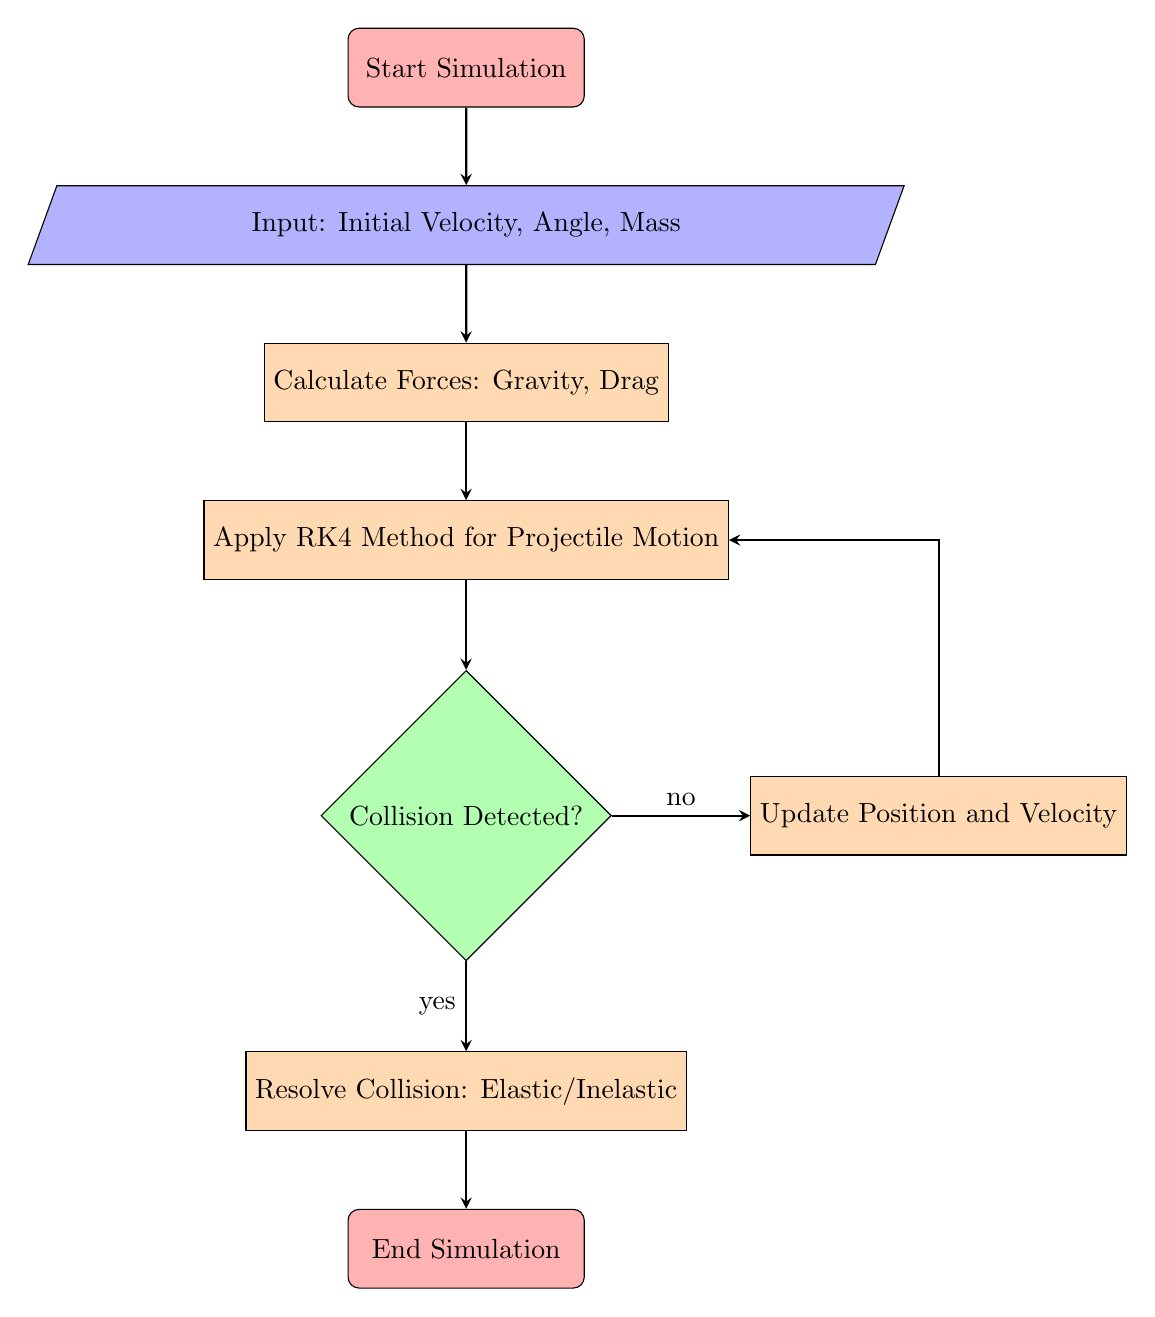
\begin{tikzpicture}[node distance=2cm]
\node (start) [startstop] {Start Simulation};
\node (input) [io, below of=start] {Input: Initial Velocity, Angle, Mass};
\node (forces) [process, below of=input] {Calculate Forces: Gravity, Drag};
\node (RK4) [process, below of=forces] {Apply RK4 Method for Projectile Motion};
\node (collision) [decision, below of=RK4, yshift=-1.5cm] {Collision Detected?};
\node (update) [process, right of=collision, xshift=4cm] {Update Position and Velocity};
\node (resolve) [process, below of=collision, yshift=-1.5cm] {Resolve Collision: Elastic/Inelastic};
\node (end) [startstop, below of=resolve] {End Simulation};

\draw [arrow] (start) -- (input);
\draw [arrow] (input) -- (forces);
\draw [arrow] (forces) -- (RK4);
\draw [arrow] (RK4) -- (collision);
\draw [arrow] (collision) -- node[anchor=east] {yes} (resolve);
\draw [arrow] (resolve) -- (end);
\draw [arrow] (collision) -- node[anchor=south] {no} (update);
\draw [arrow] (update) |- (RK4);
\end{tikzpicture}

\subsection{Appendix C: Issues List}
\begin{tabular}{|p{0.2\textwidth}|p{0.6\textwidth}|p{0.2\textwidth}|}
    \hline
    \textbf{Issue ID} & \textbf{Description} & \textbf{Resolution} \\
    \hline
    001 & some inaccuracy found as projectile trajectory predictions at edge cases when used with Euler & Implemented improved numerical integration technique Like RK4 for edge cases. \\
    \hline
\end{tabular}


\subsection{Appendix D: Compliance Requirements}
\begin{itemize}
    \item The game must comply with the General Data Protection Regulation (GDPR) for users in the European Union.
    \item Accessibility features must align with the Web Content Accessibility Guidelines (WCAG) 2.1 for inclusivity.
    % Add more compliance requirements here
\end{itemize}


\subsection{Appendix E: Detailed RK4 Method Explanation}
The Runge-Kutta 4th Order Method is used to approximate the solutions to the ordinary differential equations governing projectile motion in "Angry Birds Alike". Here is a step-by-step breakdown of the RK4 method:

\subsection{Projectile Distance by Launch Angle}
The following chart illustrates the distance traveled by a projectile over a range of launch angles at a fixed initial speed, demonstrating the optimal angle for maximum distance.

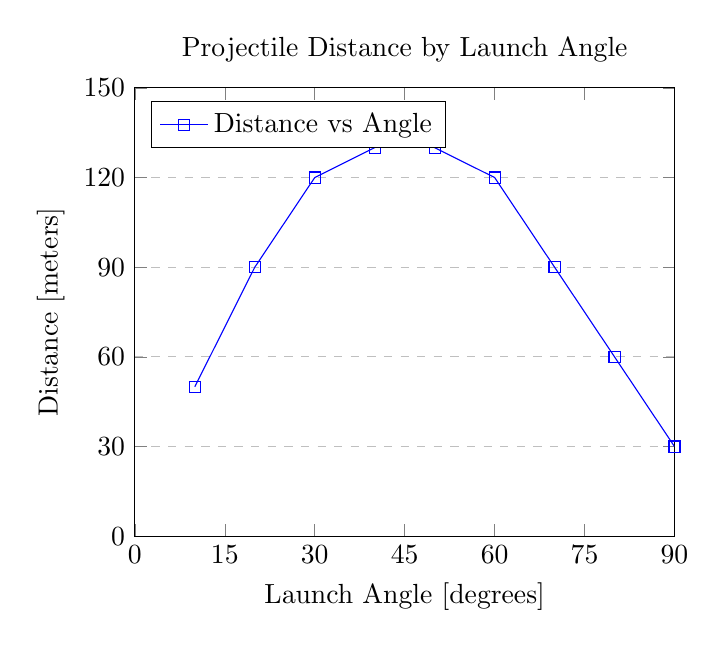
\begin{tikzpicture}
\begin{axis}[
    title={Projectile Distance by Launch Angle},
    xlabel={Launch Angle [degrees]},
    ylabel={Distance [meters]},
    xmin=0, xmax=90,
    ymin=0, ymax=150,
    xtick={0,15,30,45,60,75,90},
    ytick={0,30,60,90,120,150},
    legend pos=north west,
    ymajorgrids=true,
    grid style=dashed,
]

\addplot[
    color=blue,
    mark=square,
    ]
    coordinates {
    (10,50)(20,90)(30,120)(40,130)(45,135)(50,130)(60,120)(70,90)(80,60)(90,30)
    };
    \legend{Distance vs Angle}

\end{axis}
\end{tikzpicture}


\section{References}
The following sources were referenced in the preparation of this Software Requirements Specification:

\begin{enumerate}
    \item SFML Documentation. (n.d.). \textit{Simple and Fast Multimedia Library}. Retrieved from \url{https://www.sfml-dev.org/documentation/}
    \item Boost.odeint Documentation. (n.d.). \textit{odeint - Solving Ordinary Differential Equations}. Retrieved from \url{https://www.boost.org/doc/libs/1_75_0/libs/numeric/odeint/doc/html/index.html}
    \item Hairer, E., Nørsett, S. P., \& Wanner, G. (1993). \textit{Solving Ordinary Differential Equations I: Nonstiff Problems}. Springer Series in Computational Mathematics.
    \item Rovio Entertainment Corporation. (n.d.). \textit{Angry Birds}. Retrieved from \url{https://www.angrybirds.com/}
    \item Serway, R. A., \& Jewett, J. W. (2018). \textit{Physics for Scientists and Engineers}. Cengage Learning.
    \item Real-Time Collision Detection. (2005). Christer Ericson, \textit{Real-Time Collision Detection}. Morgan Kaufmann Publishers.
    \item Butcher, J. C. (2008). \textit{Numerical Methods for Ordinary Differential Equations}. John Wiley \& Sons.
    \item The Physics Classroom. (n.d.). \textit{Momentum and Its Conservation}. Retrieved from \url{https://www.physicsclassroom.com/class/momentum}
    \item Kiusalaas, J. (2013). \textit{Numerical Methods in Engineering with Python 3}. Cambridge University Press.
    \item OpenGL Wiki. (n.d.). \textit{Main Page}. Retrieved from \url{https://www.khronos.org/opengl/wiki/Main_Page}
\end{enumerate}


\end{document}